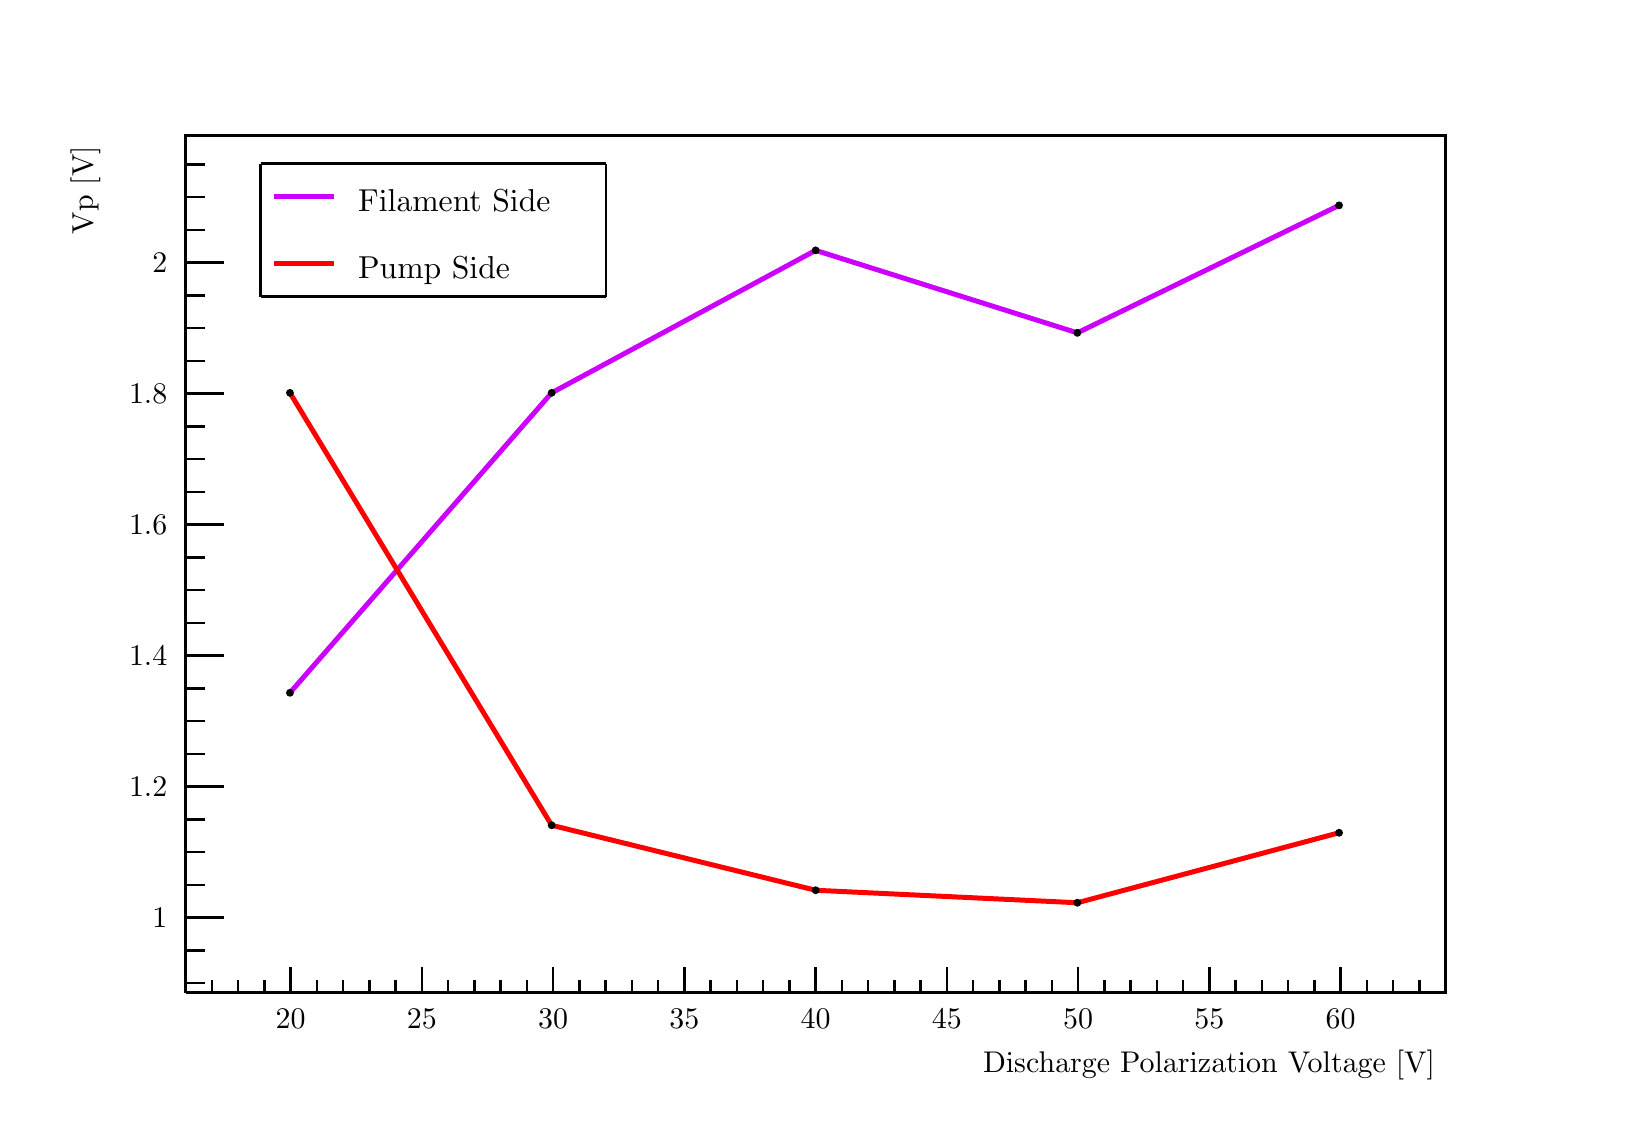
\begin{tikzpicture}
\pgfdeclareplotmark{cross} {
\pgfpathmoveto{\pgfpoint{-0.3\pgfplotmarksize}{\pgfplotmarksize}}
\pgfpathlineto{\pgfpoint{+0.3\pgfplotmarksize}{\pgfplotmarksize}}
\pgfpathlineto{\pgfpoint{+0.3\pgfplotmarksize}{0.3\pgfplotmarksize}}
\pgfpathlineto{\pgfpoint{+1\pgfplotmarksize}{0.3\pgfplotmarksize}}
\pgfpathlineto{\pgfpoint{+1\pgfplotmarksize}{-0.3\pgfplotmarksize}}
\pgfpathlineto{\pgfpoint{+0.3\pgfplotmarksize}{-0.3\pgfplotmarksize}}
\pgfpathlineto{\pgfpoint{+0.3\pgfplotmarksize}{-1.\pgfplotmarksize}}
\pgfpathlineto{\pgfpoint{-0.3\pgfplotmarksize}{-1.\pgfplotmarksize}}
\pgfpathlineto{\pgfpoint{-0.3\pgfplotmarksize}{-0.3\pgfplotmarksize}}
\pgfpathlineto{\pgfpoint{-1.\pgfplotmarksize}{-0.3\pgfplotmarksize}}
\pgfpathlineto{\pgfpoint{-1.\pgfplotmarksize}{0.3\pgfplotmarksize}}
\pgfpathlineto{\pgfpoint{-0.3\pgfplotmarksize}{0.3\pgfplotmarksize}}
\pgfpathclose
\pgfusepathqstroke
}
\pgfdeclareplotmark{cross*} {
\pgfpathmoveto{\pgfpoint{-0.3\pgfplotmarksize}{\pgfplotmarksize}}
\pgfpathlineto{\pgfpoint{+0.3\pgfplotmarksize}{\pgfplotmarksize}}
\pgfpathlineto{\pgfpoint{+0.3\pgfplotmarksize}{0.3\pgfplotmarksize}}
\pgfpathlineto{\pgfpoint{+1\pgfplotmarksize}{0.3\pgfplotmarksize}}
\pgfpathlineto{\pgfpoint{+1\pgfplotmarksize}{-0.3\pgfplotmarksize}}
\pgfpathlineto{\pgfpoint{+0.3\pgfplotmarksize}{-0.3\pgfplotmarksize}}
\pgfpathlineto{\pgfpoint{+0.3\pgfplotmarksize}{-1.\pgfplotmarksize}}
\pgfpathlineto{\pgfpoint{-0.3\pgfplotmarksize}{-1.\pgfplotmarksize}}
\pgfpathlineto{\pgfpoint{-0.3\pgfplotmarksize}{-0.3\pgfplotmarksize}}
\pgfpathlineto{\pgfpoint{-1.\pgfplotmarksize}{-0.3\pgfplotmarksize}}
\pgfpathlineto{\pgfpoint{-1.\pgfplotmarksize}{0.3\pgfplotmarksize}}
\pgfpathlineto{\pgfpoint{-0.3\pgfplotmarksize}{0.3\pgfplotmarksize}}
\pgfpathclose
\pgfusepathqfillstroke
}
\pgfdeclareplotmark{newstar} {
\pgfpathmoveto{\pgfqpoint{0pt}{\pgfplotmarksize}}
\pgfpathlineto{\pgfqpointpolar{44}{0.5\pgfplotmarksize}}
\pgfpathlineto{\pgfqpointpolar{18}{\pgfplotmarksize}}
\pgfpathlineto{\pgfqpointpolar{-20}{0.5\pgfplotmarksize}}
\pgfpathlineto{\pgfqpointpolar{-54}{\pgfplotmarksize}}
\pgfpathlineto{\pgfqpointpolar{-90}{0.5\pgfplotmarksize}}
\pgfpathlineto{\pgfqpointpolar{234}{\pgfplotmarksize}}
\pgfpathlineto{\pgfqpointpolar{198}{0.5\pgfplotmarksize}}
\pgfpathlineto{\pgfqpointpolar{162}{\pgfplotmarksize}}
\pgfpathlineto{\pgfqpointpolar{134}{0.5\pgfplotmarksize}}
\pgfpathclose
\pgfusepathqstroke
}
\pgfdeclareplotmark{newstar*} {
\pgfpathmoveto{\pgfqpoint{0pt}{\pgfplotmarksize}}
\pgfpathlineto{\pgfqpointpolar{44}{0.5\pgfplotmarksize}}
\pgfpathlineto{\pgfqpointpolar{18}{\pgfplotmarksize}}
\pgfpathlineto{\pgfqpointpolar{-20}{0.5\pgfplotmarksize}}
\pgfpathlineto{\pgfqpointpolar{-54}{\pgfplotmarksize}}
\pgfpathlineto{\pgfqpointpolar{-90}{0.5\pgfplotmarksize}}
\pgfpathlineto{\pgfqpointpolar{234}{\pgfplotmarksize}}
\pgfpathlineto{\pgfqpointpolar{198}{0.5\pgfplotmarksize}}
\pgfpathlineto{\pgfqpointpolar{162}{\pgfplotmarksize}}
\pgfpathlineto{\pgfqpointpolar{134}{0.5\pgfplotmarksize}}
\pgfpathclose
\pgfusepathqfillstroke
}
\definecolor{c}{rgb}{1,1,1};
\draw [color=c, fill=c] (0,0) rectangle (20,13.6103);
\draw [color=c, fill=c] (2,1.36103) rectangle (18,12.2493);
\definecolor{c}{rgb}{0,0,0};
\draw [c,line width=0.9] (2,1.36103) -- (2,12.2493) -- (18,12.2493) -- (18,1.36103) -- (2,1.36103);
\definecolor{c}{rgb}{1,1,1};
\draw [color=c, fill=c] (2,1.36103) rectangle (18,12.2493);
\definecolor{c}{rgb}{0,0,0};
\draw [c,line width=0.9] (2,1.36103) -- (2,12.2493) -- (18,12.2493) -- (18,1.36103) -- (2,1.36103);
\draw [c,line width=0.9] (2,1.36103) -- (18,1.36103);
\draw [c,line width=0.9] (3.33333,1.68768) -- (3.33333,1.36103);
\draw [c,line width=0.9] (3.66667,1.52436) -- (3.66667,1.36103);
\draw [c,line width=0.9] (4,1.52436) -- (4,1.36103);
\draw [c,line width=0.9] (4.33333,1.52436) -- (4.33333,1.36103);
\draw [c,line width=0.9] (4.66667,1.52436) -- (4.66667,1.36103);
\draw [c,line width=0.9] (5,1.68768) -- (5,1.36103);
\draw [c,line width=0.9] (5.33333,1.52436) -- (5.33333,1.36103);
\draw [c,line width=0.9] (5.66667,1.52436) -- (5.66667,1.36103);
\draw [c,line width=0.9] (6,1.52436) -- (6,1.36103);
\draw [c,line width=0.9] (6.33333,1.52436) -- (6.33333,1.36103);
\draw [c,line width=0.9] (6.66667,1.68768) -- (6.66667,1.36103);
\draw [c,line width=0.9] (7,1.52436) -- (7,1.36103);
\draw [c,line width=0.9] (7.33333,1.52436) -- (7.33333,1.36103);
\draw [c,line width=0.9] (7.66667,1.52436) -- (7.66667,1.36103);
\draw [c,line width=0.9] (8,1.52436) -- (8,1.36103);
\draw [c,line width=0.9] (8.33333,1.68768) -- (8.33333,1.36103);
\draw [c,line width=0.9] (8.66667,1.52436) -- (8.66667,1.36103);
\draw [c,line width=0.9] (9,1.52436) -- (9,1.36103);
\draw [c,line width=0.9] (9.33333,1.52436) -- (9.33333,1.36103);
\draw [c,line width=0.9] (9.66667,1.52436) -- (9.66667,1.36103);
\draw [c,line width=0.9] (10,1.68768) -- (10,1.36103);
\draw [c,line width=0.9] (10.3333,1.52436) -- (10.3333,1.36103);
\draw [c,line width=0.9] (10.6667,1.52436) -- (10.6667,1.36103);
\draw [c,line width=0.9] (11,1.52436) -- (11,1.36103);
\draw [c,line width=0.9] (11.3333,1.52436) -- (11.3333,1.36103);
\draw [c,line width=0.9] (11.6667,1.68768) -- (11.6667,1.36103);
\draw [c,line width=0.9] (12,1.52436) -- (12,1.36103);
\draw [c,line width=0.9] (12.3333,1.52436) -- (12.3333,1.36103);
\draw [c,line width=0.9] (12.6667,1.52436) -- (12.6667,1.36103);
\draw [c,line width=0.9] (13,1.52436) -- (13,1.36103);
\draw [c,line width=0.9] (13.3333,1.68768) -- (13.3333,1.36103);
\draw [c,line width=0.9] (13.6667,1.52436) -- (13.6667,1.36103);
\draw [c,line width=0.9] (14,1.52436) -- (14,1.36103);
\draw [c,line width=0.9] (14.3333,1.52436) -- (14.3333,1.36103);
\draw [c,line width=0.9] (14.6667,1.52436) -- (14.6667,1.36103);
\draw [c,line width=0.9] (15,1.68768) -- (15,1.36103);
\draw [c,line width=0.9] (15.3333,1.52436) -- (15.3333,1.36103);
\draw [c,line width=0.9] (15.6667,1.52436) -- (15.6667,1.36103);
\draw [c,line width=0.9] (16,1.52436) -- (16,1.36103);
\draw [c,line width=0.9] (16.3333,1.52436) -- (16.3333,1.36103);
\draw [c,line width=0.9] (16.6667,1.68768) -- (16.6667,1.36103);
\draw [c,line width=0.9] (3.33333,1.68768) -- (3.33333,1.36103);
\draw [c,line width=0.9] (3,1.52436) -- (3,1.36103);
\draw [c,line width=0.9] (2.66667,1.52436) -- (2.66667,1.36103);
\draw [c,line width=0.9] (2.33333,1.52436) -- (2.33333,1.36103);
\draw [c,line width=0.9] (16.6667,1.68768) -- (16.6667,1.36103);
\draw [c,line width=0.9] (17,1.52436) -- (17,1.36103);
\draw [c,line width=0.9] (17.3333,1.52436) -- (17.3333,1.36103);
\draw [c,line width=0.9] (17.6667,1.52436) -- (17.6667,1.36103);
\draw [anchor=base] (3.33333,0.911891) node[scale=1.08185, color=c, rotate=0]{20};
\draw [anchor=base] (5,0.911891) node[scale=1.08185, color=c, rotate=0]{25};
\draw [anchor=base] (6.66667,0.911891) node[scale=1.08185, color=c, rotate=0]{30};
\draw [anchor=base] (8.33333,0.911891) node[scale=1.08185, color=c, rotate=0]{35};
\draw [anchor=base] (10,0.911891) node[scale=1.08185, color=c, rotate=0]{40};
\draw [anchor=base] (11.6667,0.911891) node[scale=1.08185, color=c, rotate=0]{45};
\draw [anchor=base] (13.3333,0.911891) node[scale=1.08185, color=c, rotate=0]{50};
\draw [anchor=base] (15,0.911891) node[scale=1.08185, color=c, rotate=0]{55};
\draw [anchor=base] (16.6667,0.911891) node[scale=1.08185, color=c, rotate=0]{60};
\draw [anchor= east] (18,0.446418) node[scale=1.08185, color=c, rotate=0]{Discharge Polarization Voltage [V]};
\draw [c,line width=0.9] (2,1.36103) -- (2,12.2493);
\draw [c,line width=0.9] (2.48,2.3139) -- (2,2.3139);
\draw [c,line width=0.9] (2.24,2.72986) -- (2,2.72986);
\draw [c,line width=0.9] (2.24,3.14582) -- (2,3.14582);
\draw [c,line width=0.9] (2.24,3.56178) -- (2,3.56178);
\draw [c,line width=0.9] (2.48,3.97774) -- (2,3.97774);
\draw [c,line width=0.9] (2.24,4.39369) -- (2,4.39369);
\draw [c,line width=0.9] (2.24,4.80965) -- (2,4.80965);
\draw [c,line width=0.9] (2.24,5.22561) -- (2,5.22561);
\draw [c,line width=0.9] (2.48,5.64157) -- (2,5.64157);
\draw [c,line width=0.9] (2.24,6.05753) -- (2,6.05753);
\draw [c,line width=0.9] (2.24,6.47349) -- (2,6.47349);
\draw [c,line width=0.9] (2.24,6.88944) -- (2,6.88944);
\draw [c,line width=0.9] (2.48,7.3054) -- (2,7.3054);
\draw [c,line width=0.9] (2.24,7.72136) -- (2,7.72136);
\draw [c,line width=0.9] (2.24,8.13732) -- (2,8.13732);
\draw [c,line width=0.9] (2.24,8.55328) -- (2,8.55328);
\draw [c,line width=0.9] (2.48,8.96923) -- (2,8.96923);
\draw [c,line width=0.9] (2.24,9.38519) -- (2,9.38519);
\draw [c,line width=0.9] (2.24,9.80115) -- (2,9.80115);
\draw [c,line width=0.9] (2.24,10.2171) -- (2,10.2171);
\draw [c,line width=0.9] (2.48,10.6331) -- (2,10.6331);
\draw [c,line width=0.9] (2.48,2.3139) -- (2,2.3139);
\draw [c,line width=0.9] (2.24,1.89795) -- (2,1.89795);
\draw [c,line width=0.9] (2.24,1.48199) -- (2,1.48199);
\draw [c,line width=0.9] (2.48,10.6331) -- (2,10.6331);
\draw [c,line width=0.9] (2.24,11.049) -- (2,11.049);
\draw [c,line width=0.9] (2.24,11.465) -- (2,11.465);
\draw [c,line width=0.9] (2.24,11.8809) -- (2,11.8809);
\draw [anchor= east] (1.9,2.3139) node[scale=1.08185, color=c, rotate=0]{1};
\draw [anchor= east] (1.9,3.97774) node[scale=1.08185, color=c, rotate=0]{1.2};
\draw [anchor= east] (1.9,5.64157) node[scale=1.08185, color=c, rotate=0]{1.4};
\draw [anchor= east] (1.9,7.3054) node[scale=1.08185, color=c, rotate=0]{1.6};
\draw [anchor= east] (1.9,8.96923) node[scale=1.08185, color=c, rotate=0]{1.8};
\draw [anchor= east] (1.9,10.6331) node[scale=1.08185, color=c, rotate=0]{2};
\draw [anchor= east] (0.726934,12.2493) node[scale=1.08185, color=c, rotate=90]{Vp [V]};
\definecolor{c}{rgb}{0.8,0,1};
\draw [c,line width=1.8] (3.32378,5.17033) -- (6.64756,8.97963) -- (10,10.7891) -- (13.3238,9.74149) -- (16.6476,11.3604);
\definecolor{c}{rgb}{0,0,0};
\foreach \P in {(3.32378,5.17033), (6.64756,8.97963), (10,10.7891), (13.3238,9.74149), (16.6476,11.3604)}{\draw[mark options={color=c,fill=c},mark size=1.201201pt,mark=*] plot coordinates {\P};}
\definecolor{c}{rgb}{1,0,0};
\draw [c,line width=1.8] (3.32378,8.97963) -- (6.64756,3.48789) -- (10,2.66254) -- (13.3238,2.50382) -- (16.6476,3.39266);
\definecolor{c}{rgb}{0,0,0};
\foreach \P in {(3.32378,8.97963), (6.64756,3.48789), (10,2.66254), (13.3238,2.50382), (16.6476,3.39266)}{\draw[mark options={color=c,fill=c},mark size=1.201201pt,mark=*] plot coordinates {\P};}
\definecolor{c}{rgb}{1,1,1};
\draw [color=c, fill=c] (2.95129,10.2006) rectangle (7.33524,11.8911);
\definecolor{c}{rgb}{0,0,0};
\draw [c,line width=0.9] (2.95129,10.2006) -- (7.33524,10.2006);
\draw [c,line width=0.9] (7.33524,10.2006) -- (7.33524,11.8911);
\draw [c,line width=0.9] (7.33524,11.8911) -- (2.95129,11.8911);
\draw [c,line width=0.9] (2.95129,11.8911) -- (2.95129,10.2006);
\draw [anchor=base west] (4.04728,11.2783) node[scale=1.14549, color=c, rotate=0]{Filament Side};
\definecolor{c}{rgb}{0.8,0,1};
\draw [c,line width=1.8] (3.11569,11.4685) -- (3.88288,11.4685);
\definecolor{c}{rgb}{0,0,0};
\draw [anchor=base west] (4.04728,10.433) node[scale=1.14549, color=c, rotate=0]{Pump Side};
\definecolor{c}{rgb}{1,0,0};
\draw [c,line width=1.8] (3.11569,10.6232) -- (3.88288,10.6232);
\end{tikzpicture}
